\documentclass[11pt]{article}
 
\usepackage[margin=.95in]{geometry} 
\usepackage{amsmath,amsthm,amssymb, graphicx, multicol, array}
 
\newcommand{\N}{\mathbb{N}}
\newcommand{\Z}{\mathbb{Z}}
 

\begin{document}
 
\title{Homework 3}
\author{Juliette Franqueville\\
}
\maketitle

\subsection*{(2) Show that binomial and negative binomial distributions belong to exponential families}

For the binomial distribution:

\begin{align*}
    P(y) &= {n \choose y}p^y(1-p)^{n-y}\\
    &=  {n \choose y}\text{exp}\{\text{log}[p^y(1-p)^{n-y}]\}\\
     &=  {n \choose y}\text{exp}\{y\text{log}p +(n-y)\text{log}(1-p)\}\\
     &=  {n \choose y}\text{exp}\left \{y\text{log}\frac{p}{1-p} +n\text{log}(1-p)\right \}
\end{align*}

We have 
\begin{align*}
    \theta &= \text{log}\frac{p}{1-p} \\
    \text{exp}\theta &= \frac{p}{1-p} \\
     \text{exp}\theta(1-p) &=p \\
      \text{exp}\theta(1-p) &=p \\
      \text{exp}\theta - p\text{exp}\theta &=p \\
            \text{exp}  &=p(1+\text{exp}\theta) \\
             p  &=\text{exp}\theta/(1+\text{exp}\theta) \\
               1-p  &=1-\text{exp}\theta/(1+\text{exp}\theta) \\
               &=1/(1+\text{exp}\theta) 
\end{align*}
So:

\begin{align*}
    P(y) &=  {n \choose y}\text{exp}\left \{y\text{log}\frac{p}{1-p} +n\text{log}(1-p)\right \}\\
    &=  {n \choose y}\text{exp}\left \{y\text{log}\frac{p}{1-p} -n\text{log}[1+\text{exp}\theta]\right \}
\end{align*}

So we have $h(y) = {n \choose y}$, $\theta &= \text{log}\frac{p}{1-p}$ and $\psi(\theta) = n\text{log}[1+\text{exp}\theta]$

For the negative binomial distribution:

\begin{align*}
    P(y) &= {y+r-1 \choose y}(1-p)^rp^y\\
    &= {y+r-1 \choose y}\text{exp} \{ \text{log}(1-p)^rp^y \}\\
     &= {y+r-1 \choose y}\text{exp} \{ r\text{log}(1-p) + y\text{log}p \}
\end{align*}
We have:
\begin{align*}
    \theta &= \text{log}p\\
    p &= \text{exp}\theta\\
    1-p &= 1-\text{exp}\theta
\end{align*}

So we have $h(y) = {y+r-1 \choose y}$, $\theta &= \text{log}p$ and $\psi(\theta) =  r\text{log}(1-\text{exp}\theta)$



\subsection*{(3) Let $y \simBin(10,\theta)$. Also, let the observed value of $y = 3$. The prior is a mixture of Betas}

\subsection*{(a) Find the posterior}

Dropping constants, we have:

\begin{align*}
    P(\theta|) &\propto P(y|\theta)P(\theta)\\
   & \propto \theta^3(1-\theta)^7 \left[\frac{\theta^9(1-\theta)^{19}}{B(10, 20)} + \frac{\theta^{19}(1-\theta)^9}{B(20, 10)}\right]\\
    & \propto  \left[\frac{\theta^{12}(1-\theta)^{26}}{B(10, 20)} + \frac{\theta^{22}(1-\theta)^{16}}{B(20, 10)}\right]\\
    & \propto  \left[\frac{B(13, 27)}{B(13, 27)}\frac{\theta^{12}(1-\theta)^{26}}{B(10, 20)} +\frac{B(23, 17)}{B(23, 17)} \frac{\theta^{22}(1-\theta)^{16}}{B(20, 10)}\right]\\
     & \propto  \left[B(13, 27)\frac{Beta(13, 27)}{B(10, 20)} +B(23,  \frac{Beta(23, 17)}{B(20, 10)}\right]\\
     & \propto  \pi_1 Beta(13, 27) + \pi_2 Beta(23, 17)
\end{align*}

With $\pi_1 = \frac{\frac{B(13, 27)}{B(10, 20)}}{\frac{B(13, 27)}{B(10, 20)} + \frac{B(23, 17)}{B(20, 10)}}$ and  $\pi_2 = \frac{\frac{B(23, 17)}{B(20, 10)}}{\frac{B(13, 27)}{B(10, 20)} + \frac{B(23, 17)}{B(20, 10)}}$


\subsection*{(b) Plot the posterior superimposed on the prior}
\subsection*{(c) Compute a 90\% posterior credible interval for $\theta$}

To obtain the prior and posteriors, we sum the pdfs of the relevant betas. To find the 90\% posterior credible interval, we find value of $\theta$ corresponding to the location where the area under the pdf curve for the posterior is .05 and .95. 

\begin{figure}[!h]
    \centering
    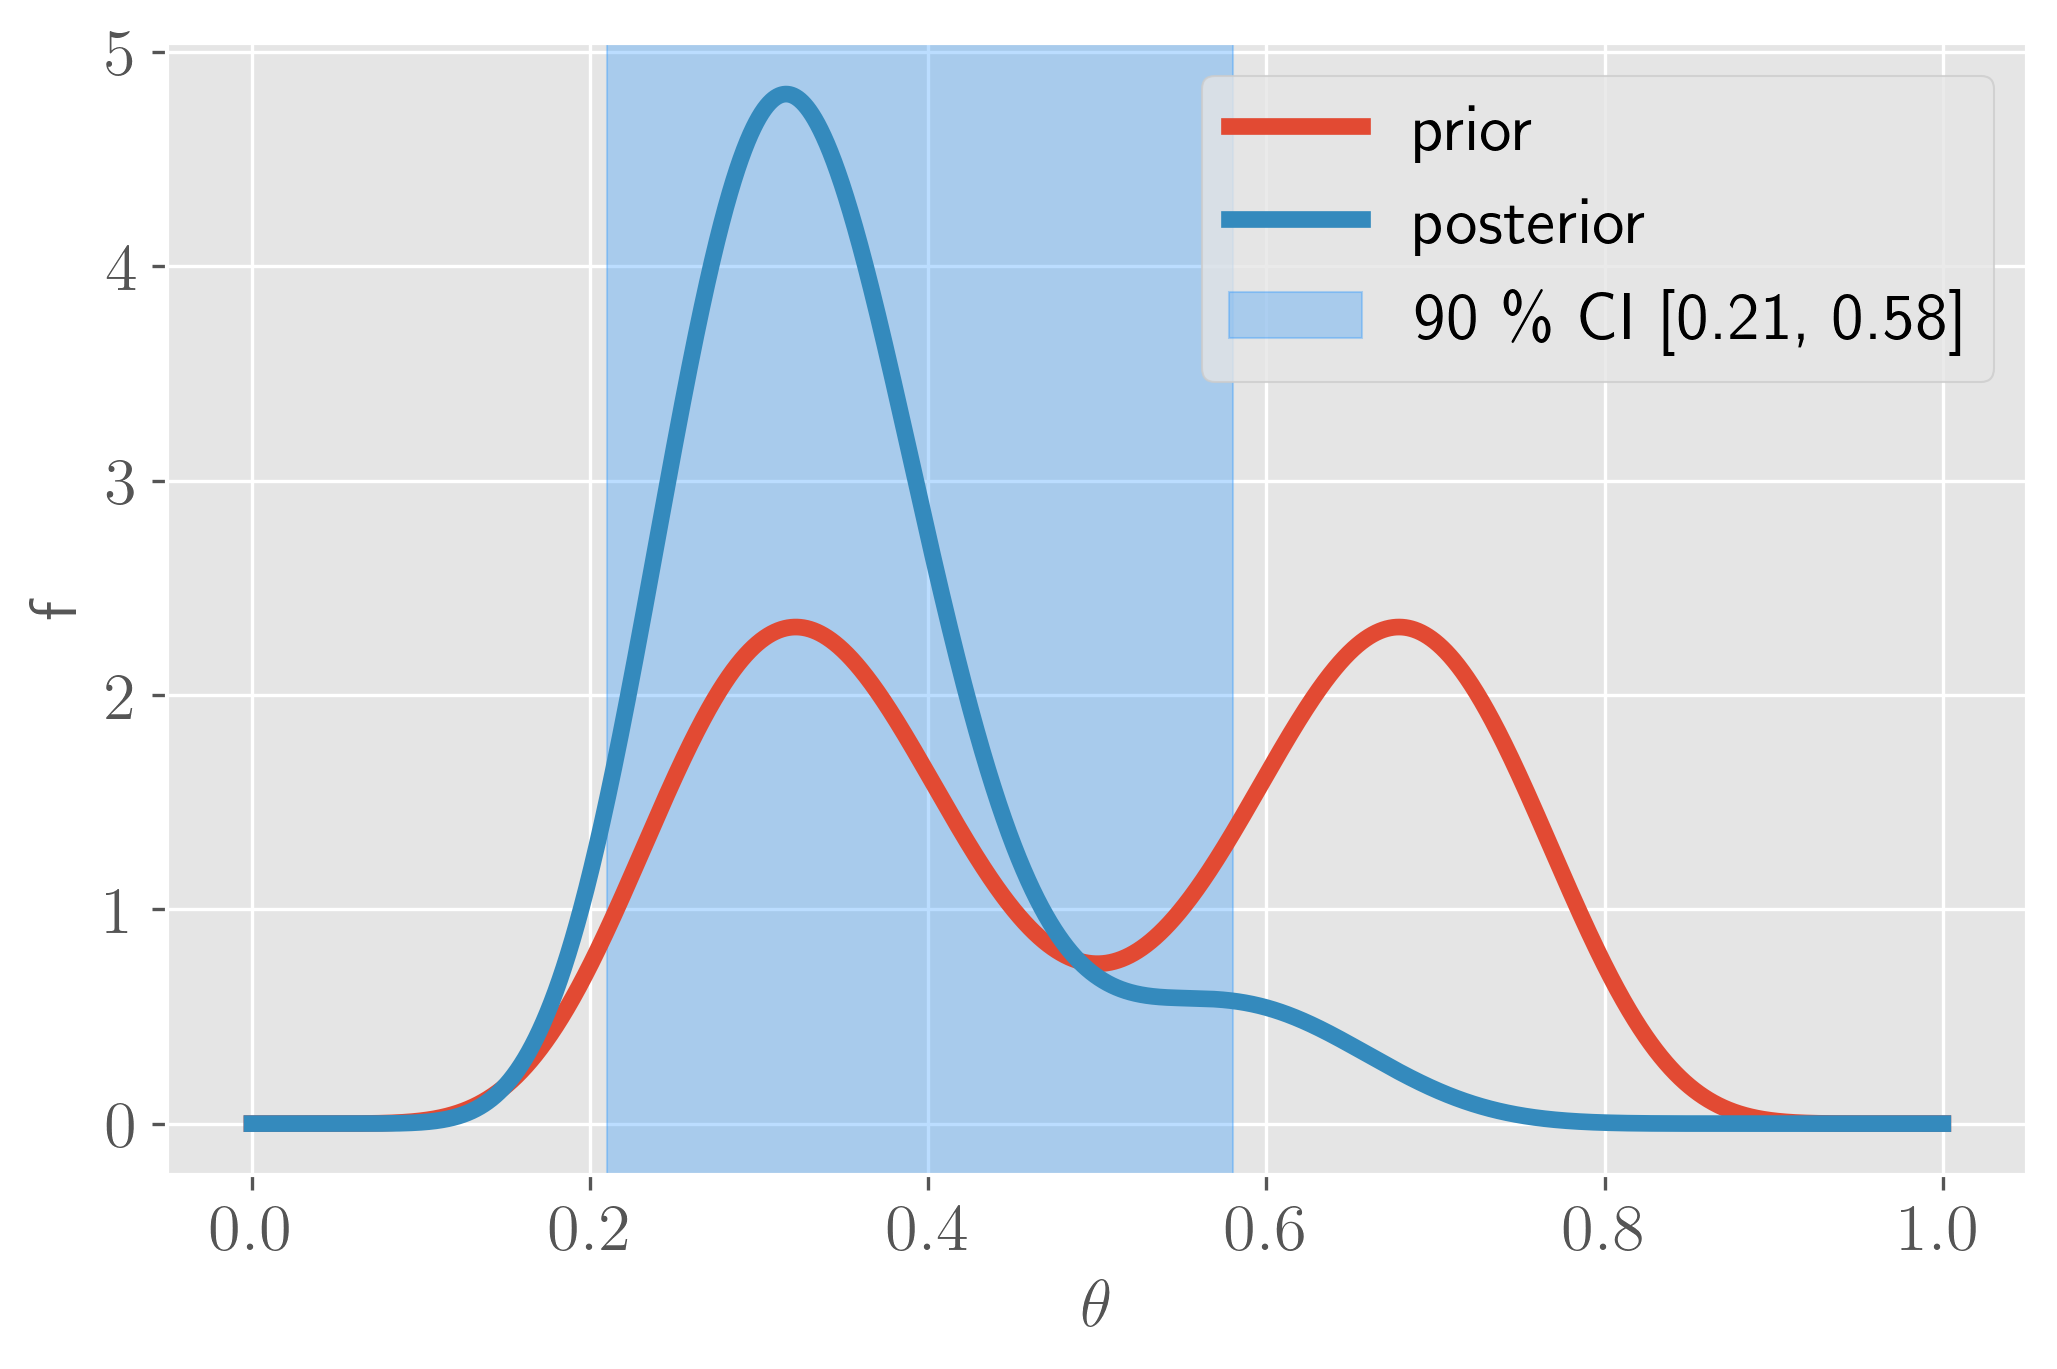
\includegraphics[scale=.6
    ]{homework_3/figures/binom.png}
    \caption{Prior / Posterior and CI}
    \label{fig:my_label}
\end{figure}

\subsection*{(4) Prove that Jeffreys’ priors satisfy the invariance principle: starting with $p(\theta) \propto |I(\theta)|^{1/2}$, show that the induced prior on $\psi = g(\theta)$, where $g$ is one-one, is
$p(\psi) \propto |I(\psi)|^{1/2}$}


\begin{align*}
    I(\psi) &= -E\left(\frac{\partial ^2\mathcal{L}(\psi)}{\partial \psi^2}\right)\\
    &= -E\left(\frac{\partial^2\mathcal{L}(\psi)}{\partial \theta^2} \left[\frac{\partial \theta}{\partial \psi}\right]^2 + \frac{\partial \mathcal{L}}{\partial \theta} \frac{\partial ^2\psi}{\partial \theta^2}\right)\\
     &= -\left[\frac{\partial \theta}{\partial \psi}\right]^2E\left(\frac{\partial^2\mathcal{L}(\psi)}{\partial \theta^2}\right)  -\frac{\partial ^2\psi}{\partial \theta^2}E\left(\frac{\partial \mathcal{L}(\psi)}{\partial \theta} \right)
\end{align*}

$E\left(\frac{\partial \mathcal{L}(\phi)}{\partial \theta} \right)$ is the score and its expectation is 0:

\begin{align*}
    E\left(\frac{\partial \mathcal{L}(\psi)}{\partial \theta} \right) &= \int^{\infty}_{-\infty} f(y|\psi)  \frac{\partial \mathcal{L}(\psi)}{\partial \theta} dy\\
    &= \int^{\infty}_{-\infty} f(y|\psi)  \frac{\partial \text{log}f(y|\psi) }{\partial \theta} dy\\
    &= \int^{\infty}_{-\infty} f(y|\psi) \frac{1}{f(y|\psi) }  \frac{\partial f(y|\psi) }{\partial \theta} dy\\
     &= \frac{\partial }{\partial \theta} \int^{\infty}_{-\infty}f(y|\psi) dy \\
     & = \frac{\partial }{\partial \theta} (1) = 0
\end{align*}

So we have:

\begin{align*}
    I(\psi) &=-\left[\frac{\partial \theta}{\partial \psi}\right]^2E\left(\frac{\partial^2\mathcal{L}(\psi)}{\partial \theta^2}\right)  \\
    &= \left[\frac{\partial \theta}{\partial \psi}\right]^2 I(\theta)\\
\end{align*}

Then, 

\begin{align*}
    P(\psi) &= P(\theta) \left|\frac{\partial \psi}{\partial \theta}\right|^{-1}\\
    &= |I(\theta)|^{1/2}\left|\frac{\partial \psi}{\partial \theta}\right|^{-1}\\
     &= \left|I(\psi)\left[\frac{\partial \psi}{\partial \theta}\right]^2\right|^{1/2}\left|\frac{\partial \psi}{\partial \theta}\right|^{-1}\\
     &= |I(\psi)|^{1/2}
\end{align*}
\subsection*{(5) For the Poisson likelihood model $y_1\ldots y_n
 \sim Poisson(\lambda)$, Jeffrey’s (improper) prior was derived in class. Compute the corresponding posterior. Is it proper?}

Jeffreys' prior for the Poisson distribution is $\lambda \propto \lambda^{-1/2}$

We have:

\begin{align*}
    P(\lambda|y) &\propto P(y|\lambda)P(\lambda)\\
    &\propto \prod \lambda^y\text{exp}\{-\lambda\}\lambda^{-1/2}\\
    &\propto  \lambda^{1/2 + \sum y_i - 1} \text{exp}\{-\lambda n\}\\
    &= Ga\left(1/2 + \sum y_i, n \right)
    \end{align*}
    
Since the posterior is a Gamma distribution, it is proper (integrates to 1).



\end{document}
